%=========================================
% 	   Cloud Native     		 =
%=========================================
\chapter{Cloud-Native}

Im zweiten Kapitel gehen wir auf die Definition von Cloud-Native Architekturen ein, grenzen diese von anderen Absätzen ab und betrachten wichtige Eigenschaften. Abschließend beschäftigen wir uns mit den Vor-und Nachteilen und den typischen Einsatzgebieten.

\section{Cloud-Computing}
Bevor wir uns mit Cloud-Native Architekturen auseinandersetzten können, müssen wir uns zuerst mit dem Cloud-Computing beschäftigen, da es die Basis für diese Architekturen bildet und sie maßgeblich beeinflusst. Die \ac{NIST} Definition von Cloud-Computing enthält die wichtigsten Merkmale.\\
\\
\glqq Cloud computing is a model for enabling ubiquitous, convenient, on-demand network access to a shared pool of configurable computing resources (e.g., networks, servers, storage, applications, and services) that can be rapidly provisioned and released with minimal management effort or service provider interaction. This cloud model is composed of five essential characteristics, three service models, and four deployment models.\grqq{} \cite{Nist}\\
\\
Entscheidend für Cloud-Native ist nun die schnelle Bereitstellung von Ressourcen, denn dies eröffnet neue Möglichkeiten hinsichtlich der Skalierbarkeit und hat dadurch einen starken Einfluss auf die Architekturen.

\section{Definition Cloud-Native}
Was genau Cloud-Native ist und wie man es definieren kann ist schwierig, da der Begriff noch relativ neu ist. Eine erste Version einer Definition kommt von der \ac{CNCF}, einer Organisation, die als Vorreiter in Sachen Cloud-Native gilt.\\
\\
\textbf{CNCF Cloud Native Definition v1.0}\\
\\
\glqq Cloud-Native Technologien ermöglichen es Unternehmen, skalierbare Anwendungen in modernen, dynamischen Umgebungen zu implementieren und zu betreiben. Dies können öffentliche, private und Hybrid-Clouds sein. Best Practices, wie Container, Service-Meshs, Microservices, immutable Infrastruktur und deklarative \ac{API}, unterstützen diesen Ansatz.
\\
Die zugrundeliegenden Techniken ermöglichen die Umsetzung von entkoppelten Systemen, die belastbar, handhabbar und beobachtbar sind. Kombiniert mit einer robusten Automatisierung können Softwareentwickler mit geringem Aufwand flexibel und schnell auf Änderungen reagieren.
\\
Die Cloud Native Computing Foundation fördert die Akzeptanz dieser Paradigmen durch die Ausgestaltung eines Open Source Ökosystems aus herstellerneutralen Projekten. Wir demokratisieren modernste und innovative Softwareentwicklungs-Patterns, um diese Innovationen für alle zugänglich zu machen.\grqq{} \cite{CNCF}\\
\\
Diese Definition lässt gewollt viel Spielraum zur Interpretation, jedoch stechen ein paar wichtige Merkmale heraus. Diese sind insbesondere Entkopplung, Belastbarkeit, robuste Automatisierung und Skalierbarkeit. Die CNCF hat diese Definition als Version 1.0 markiert, was darauf schließen lässt, das Änderungen oder Erweiterungen erwartet werden.

\section{Microservices}
Microservices sind in Cloud-Native Systemen zum Erstellen von Anwendungen ein beliebter Architekturstil. Bei dieser Architektur besteht die Software aus kleinen, unabhängigen Services bzw. Modulen, die über definierte APIs kommunizieren. Jeder Service kann unabhängig von anderen Services entwickelt und bereitgestellt werden, ohne die Funktionalität anderer Services zu beeinträchtigen. Den Aufbau einer beispielhaften Microservice-Architektur sowie die Darstellung der einzelnen unabhängigen Services sind in Abbildung \ref{micro} zu sehen.\\
\begin{figure}[bth] 
	\centering
	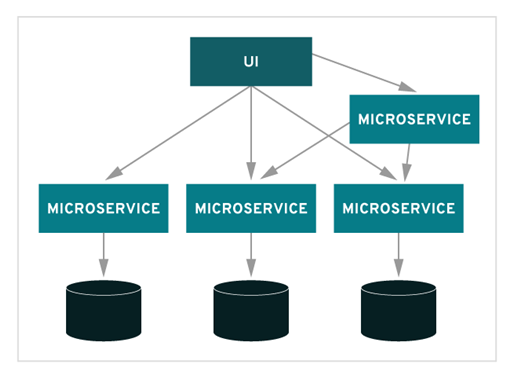
\includegraphics[width=0.6\textwidth]{Graphics/Microservice.png}
	\caption{Aufbau einer Microservice-Architektur}
	\label{micro}
	\cite{microBild}
\end{figure}\\
Durch die Eigenständigkeit besitzt jeder Komponentenservice seinen eigenen Code sowie seine eigene Implementierung. Jede einzelne Komponente ist auf eine Reihe von Funktionen spezialisiert, sodass sie sich auf die Lösung eines bestimmten Problems fokussiert. Wenn ein einzelner Service (z.B. hinsichtlich des Codes) zu komplex wird, kann er in kleinere Services unterteilt werden.\\
In Cloud-Native Systemen sowie in der Microservice-Architektur ist die Skalierung ein wichtiger Bestandteil. Durch die Existenz der einzelnen Services können diese je nach Nachfrage unabhängig voneinander skaliert werden. Dadurch können Subsysteme, die mehr Ressourcen benötigen hochskaliert werden, ohne die gesamte Anwendung hochzuskalieren.\\
Eine weitere Eigenschaft ist die Flexibilität. Durch die Unabhängigkeit der einzelnen Services wird auch deren Verwaltung vereinfacht. Bei einer Erweiterung sowie Fehlerbehebung der Anwendung muss nur der entsprechende Service verändert werden. Dies führt dazu, dass nicht die gesamte Anwendung erneut bereitgestellt werden muss.\\
Durch die einfache Bereitstellung können z.B. neue Konzepte ausprobiert und auch schnell wieder rückgängig gemacht werden. Auf Grund der möglichen Experimente entstehen niedrige Ausfallkosten, die Aktualisierung des Codes wird erleichtert und vereinfacht das Hinzufügen neuer Funktionen.\cite{microservice}
\section{Container}
Auch Container sind ein wesentlicher Bestandteil von Cloud-Native Systemen.\\
Ein Container ist eine Standard-Software-Einheit, die den Code und seine Abhängigkeiten verpackt, sodass Anwendungen von ihrer Ausführungsumgebung abstrahiert werden. Mit dieser Entkopplung können containerbasierte Anwendungen schnell, zuverlässig bereitgestellt und von einer beliebigen Umgebung, wie z.B. in einer öffentlichen Cloud, ausgeführt werden. In Abbildung \ref{container} ist der Aufbau einer containerbasierten Anwendung zu sehen.\\
\begin{figure}[bth] 
	\centering
	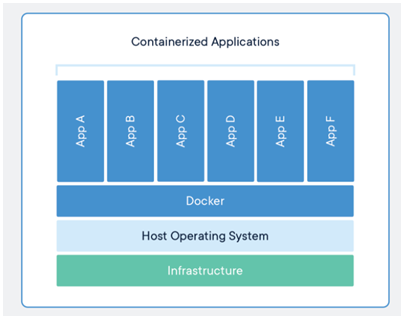
\includegraphics[width=0.6\textwidth]{Graphics/Container.png}
	\caption{Aufbau einer containerbasierte Anwendung}
	\label{container}
	\cite{container}
\end{figure}\\
Im Gegensatz zu virtuellen Maschinen wird bei der Containerisierung weniger Speicherplatz benötigt. Hierbei handelt es sich um eine Virtualisierung auf Betriebssystemebene, da die Container direkt auf dem Kernel des Betriebssystems ausgeführt werden. Container teilen sich den Kernel des Betriebssystems, sodass sie schneller starten und im Vergleich zu einem vollständigen Betriebssystem nur einen Bruchteil an Speicher verwenden.\\
Container haben eine hohe Portabilität, sodass sie überall ausgeführt werden können. Die Softwarepakete enthalten alle Elemente, die zur Ausführung in einer beliebigen Umgebung erforderlich sind.\\
Auch bei der Containerisierung ist die Skalierbarkeit eine wichtige Eigenschaft. Denn hier besteht die Möglichkeit, dass die einzelnen Container je nach Ressourcenbedarf schnell gestartet sowie angehalten werden können. Zudem laufen sie isoliert von anderen Anwendungen.\cite{container}\\
\\                                                                                   
Es gibt verschiedene Containerformate, mit deren Hilfe eine Anwendungsbereitstellung durch Containerisierung erleichtert wird. Bekannte Containerformate sind z.B. Docker und Kubernetes.\\
Docker ist ein beliebtes Open-Source-Containerformat zur Automatisierung der Bereitstellung von Anwendungen, die z.B. in der Cloud ausgeführt werden können. Docker verpackt die Software mit seinen Abhängigkeiten und alles was zur Ausführung benötigt wird in Container.\\
Wenn Anwendungen immer größer werden und die Betreibung immer komplexer wird, ist das Orchestrierungssystem Kubernetes hilfreich.\\
Kubernetes ist ein Open-Source-Orchestrierungssystem zur Automatisierung z.B. zur Verwaltung, Platzierung und Skalierung von Container.\cite{kubernetes}
                   
\section{Abgrenzungen}
In diesem Abschnitt wird die monolithische Architektur im Gegensatz zur Microservice Architektur abgegrenzt. Darüber hinaus werden virtuelle Maschinen einer containerbasierten Anwendung gegenübergestellt.

\subsection{Monolithische Architektur}
Bei einer monolithischen Architektur sind die Prozesse eng miteinander verbunden und werden als einziger Service ausgeführt. Wenn ein Fehler auftritt, muss im Gegensatz zu der Microservice Architektur, die gesamte Anwendung skaliert werden und nicht nur der betroffene Service. Das Hinzufügen und Verbessern von Funktionen sowie das Umsetzen neuer Konzepte kann bei der monolithischen Architektur je nach Aufbau der Implementierung mit zunehmender Codebasis komplexer werden. Die Anwendungsverfügbarkeit ist im Gegensatz zu den Microservices risikoreicher. Bei der monolithischen Architektur sind die einzelne Prozesse abhängig voneinander und eng miteinander verbunden, sodass die Wahrscheinlichkeit für einen Prozessausfall erhöht wird.\\
In Abbildung \ref{mono} sind die beschriebenen Aufbauten der monolithischen Architektur und der Microservice Architektur vergleichend dargestellt.
\begin{figure}[bth] 
	\centering
	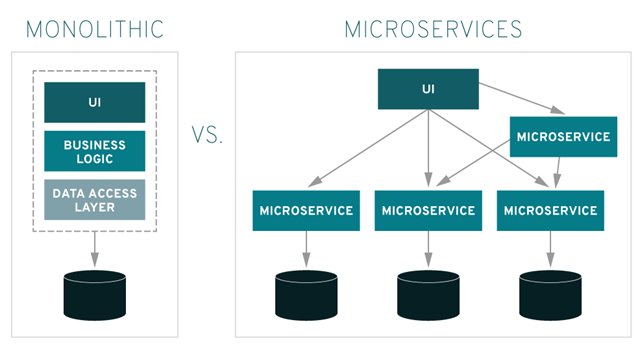
\includegraphics[width=0.9\textwidth]{Graphics/monoVsMicro.png}
	\caption{Vergleich der monolithischen Architektur und der Microservice Architektur}
	\label{mono}
	\cite{microBild}
\end{figure}\\
\subsection{Virtuelle Maschinen}
Im Gegensatz zu Container, sind virtuelle Maschinen eine Virtualisierung der gesamten Hardware bzw. Abstraktion der physischen Hardware, die einen Server in viele Server wandelt. In Abbildung \ref{vm} ist der Aufbau einer containerbasierten Anwendung im Vergleich zu einer virtuellen Maschine dargestellt.
\begin{figure}[bth] 
	\centering
	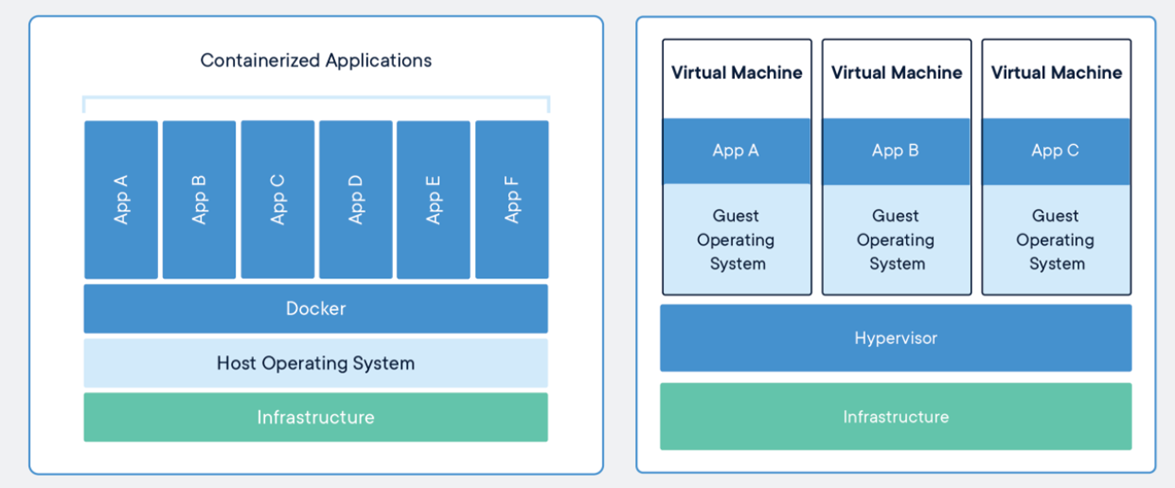
\includegraphics[width=0.9\textwidth]{Graphics/containerVsVm.png}
	\caption{Vergleich einer containerbasierten Anwendung zu einer virtuellen Maschine}
	\label{vm}
	\cite{container}
\end{figure}\\
Bei einer virtuellen Maschine ermöglicht der Hypervisor die Ausführung mehrerer virtuellen Maschinen auf einer einzigen Maschine. Jede virtuelle Maschine enthält eine vollständige Kopie eines Betriebssystems, der Anwendung, notwendiger Binärdateien und Bibliotheken. In Abbildung \ref{vm} sind drei Gastbetriebssysteme zu sehen, die alle von ihrem Hypervisor kontrolliert werden. Jedes System benötigt seine eigenen CPU- und Speicherressourcen sowie seine eigene Kopie verschiedener Binärdateien und Bibliotheken. Dadurch benötigen virtuelle Maschinen im Vergleich zu containerbasierten Anwendungen mehr Speicher.

\section{Eigenschaften}
Als nächstes betrachten wir die am häufigsten genannten Eigenschaften von Cloud-Native Architekturen.\\
\\
\textbf{1. Globale Ebene}\\
Cloud-Native Architekturen sind oft für eine globale Ebene ausgelegt. Das impliziert z.B., dass das System mehrfach installiert werden muss und verteilte Datenbanken zum Einsatz kommen.\\
\\
\textbf{2. Skalierbarkeit}\\
Die entstehenden Architekturen sind skalierbar und können mit sehr großen Mengen von Benutzern und Daten umgehen. Dies ist besonders in Kombination mit der globalen Ebene, wenn man Synchronisation und Konsistenz betrachtet, eine große Herausforderung.\\
\\
\textbf{3. Annahme über Infrastruktur}\\
Die Annahme \glqq infrastructure is fluid\grqq{}, im Deutschen etwa Infrastruktur ist ständig änderbar, bedeutet, dass die unterliegenden Strukturen nicht konstant sind, wie es vergleichsweise bei einem Server sind, der eine bestimmte Anzahl von CPUs hat. So können z.B. Recheneinheiten (CPUs) hinzukommen oder wegfallen. Diese Annahme resultiert aus der Verwendung von Cloud-Technologien und bildet die Basis für das Entwerfen von skalierbaren Cloud Architekturen.\\
Die zweite Annahme, dass Fehler konstant auftreten, ergibt sich ebenfalls aus der Verwendung von Cloud-Technologien, denn wenn eine große Anzahl von Hard- und Softwarekomponenten verwendet werden steigt die Wahrscheinlichkeit von einem unerwarteten Ausfall. Die Architektur muss also die Möglichkeit von solchen Fehlern miteinbeziehen, denn anders ist sie nicht widerstandsfähig genug, um effektiv in einer Cloud-Umgebung zu bestehen.\\
\\
\textbf{4. Updates und Tests verlaufen unscheinbar}\\
Die Architekturen sind so entworfen, dass Systeme, ohne Verlust von Verfügbarkeit, upgedatet und getestet werden können. Techniken, die hier zum Einsatz kommen sind unter Anderem CI/CD Pipelines, die den Prozess von Entwicklung bis Installation automatisieren und Immutable Infrastructures ein Ansatz, bei dem bestehende Systeme nicht verändert werden und stattdessen eine neuere Version auf einem neuem System neu installiert wird.\\
\\
\textbf{5. Sicherheit}\\
Sicherheit spielt eine wichtige Rolle in Cloud-Native Architekturen. Die meisten Systeme bestehen aus vielen Komponenten, was eine breite Angriffsfläche bietet. Außerdem ist Autorisierung und Authentifizierung keine einfache Sache in einem entkoppelten verteilten System. Deshalb sollte Sicherheit schon beim Entwurf der Architektur eine Rolle spielen.\cite{cloud-NativeApplications}

\section{Vor- und Nachteile}
In diesem Abschnitt nennen und erklären wir einige Vor- und Nachteile von Cloud-Native Architekturen. Wir beginnen mit den Vorteilen.\\
\\
\textbf{1. Skalierbarkeit/Elastizität}\\
Aus der Kombination von entkoppelten Komponenten, Orchestrierung und Cloud-Infrastruktur entstehen effektiv skalierbare (auch elastische) Architekturen. Orchestrierung spielt dabei eine große Rolle, da ohne sie in größeren Systemen Skalierbarkeit kaum realisierbar ist.\\
\\
\textbf{2. Zuverlässigkeit/Widerstandsfähigkeit}\\
Cloud-Native Architekturen sind robust gegen Ausfälle der unterliegenden Strukturen. Hierzu werden Komponenten überwacht und bei Fehlern neu gestartet. Komponenten sind dabei oft, auch Zwecks Skalierbarkeit, redundant vorhanden. Die Orchestrierung hat auch hier eine wichtige Rolle, da sie für die Überwachung verantwortlich ist.\\
\\
\textbf{3. Änderbarkeit/Wartbarkeit}\\
Da Komponenten (wie z.B. Microservices) weitestgehend voneinander unabhängig sind, können leichter Änderungen gemacht werden, ohne andere Komponenten auch ändern zu müssen. Auch können Teile der Architektur unabhängig vom Rest installiert oder ausgetauscht werden.\\
\\
\textbf{4. Übertragbarkeit}\\
Durch die Verwendung von Containern und CI/CD Pipelines ist es möglich die Systeme in andere Umgebungen einfach zu installieren. Container ermöglichen dabei eine uniforme Umgebung für die Komponenten und sind damit unabdingbar für Cloud-Native Architekturen. \\
\\
\textbf{5. Cloud Native Computing Foundation}\\
Die CNCF ist eine Organisation, die die Entwicklung im Cloud-Native Bereich unterstützt. Sie ist ein zentraler Punkt für Informationen zu Best Practices, Standards, Open Source Projekte und Neuigkeiten im Bereich Cloud-Native.\\
\\
Die Liste der Nachteile ist zwar kurz, jedoch sind die Punkte hoch zu gewichten.\\
\\
\textbf{1. Komplexität}\\
Wie in der Vorlesung gelernt gilt für das Entwerfen von Software-Architekturen \glqq There is no silver bullet\grqq{}. Dies trifft sehr gut auf Cloud-Native Architekturen zu. Zwar existieren Tools und Herangehensweisen, die in fast allen Cloud-Native Architekturen zum Einsatz kommen, jedoch ist die schiere Auswahl an Möglichkeiten, die getroffen werden müssen, bereits eine Herausforderung.\\ 
Jede Cloud-Native Applikation ist ein verteiltes System, welches an sich schon sehr komplex werden kann. Addiert man hierzu noch Container/Container-Orchestrierung, Sicherheitsaspekte, Datenhaltung und Skalierung/Lastenverteilung kann sehr schnell der Überblick verloren gehen. Des Weiteren ist eine solche Architektur nicht einfach zu testen, installieren oder upzudaten und es müssen weitere Tools verwendet werden um dies zu bewerkstelligen.\\
Abschließend ist zu sagen, dass die hohe Komplexität aus den hohen Anforderungen (Skalierbarkeit, Erreichbarkeit, Sicherheit, etc.) stammt, die an Cloud-Native Architekturen gestellt werden und daher unvermeidbar ist. Sie steht in einem Zielkonflikt mit den anderen Anforderungen, d.h. je höher die Ansprüche desto komplexer gestaltet sich die Architektur.\\
\\
\textbf{2. Neuer Ansatz/Technologie}\\
Die CNCF treibt den Bereich Cloud-Native stark voran, dennoch ist es ein relativ neuer Ansatz. Ständig werden neue Innovationen gemacht und bestehende Tools erweitert. Dies bedeutet, dass z.B. Fachliteratur und erfahrene Entwickler kaum vorhanden sind. Jedoch wird wegen der hohe Komplexität eine hohe Expertise benötigt, was den Cloud-Native Bereich schwierig macht. \cite{Top7}

\section{Einsatzgebiete}
Cloud-Native Architekturen werden derzeit meistens für Systeme benutzt, die entweder mit vielen Daten und/oder mit einer großen Anzahl von Benutzern umgehen müssen. Also generell Systeme, die ein hohes Maß an Skalierbarkeit fordern. Besonders in den Bereichen Streaming und Big Data werden häufig Cloud-Native Architekturen verwendet.\\ 
Beispiele sind der Streaming-Dienst von Netflix sowie Produktivitätsprodukte von Google. Mittlerweile werden auch Cloud-Plattformen Angeboten (Google Cloud Platform und \ac{AWS}), die es wiederum ermöglichen Cloud-Native Applikation zu entwickeln.\\
Anzumerken ist, dass viele Unternehmen eine Migration ihrer Dienste in die Cloud vorgenommen haben, da die Möglichkeiten für Cloud basierte Systeme erst im Laufe des letzten Jahrzehnts wirklich zu einer Option wurde.